\section{Methodology}
Our proposed model structure is very similar to Seq-GAN\cite{Yu:2017:SSG:3298483.3298649} and 
it has classifier and comment generator.
\reffig{fig:structure} shows structure of our model.
On the one hand, generator create comments from post.
On the other hand, classifier evaluates two values to binary classifications with real or generated comments from generator: 
post's credibility and reality of comments.

\newpage
\begin{figure}[h]
    \centering
    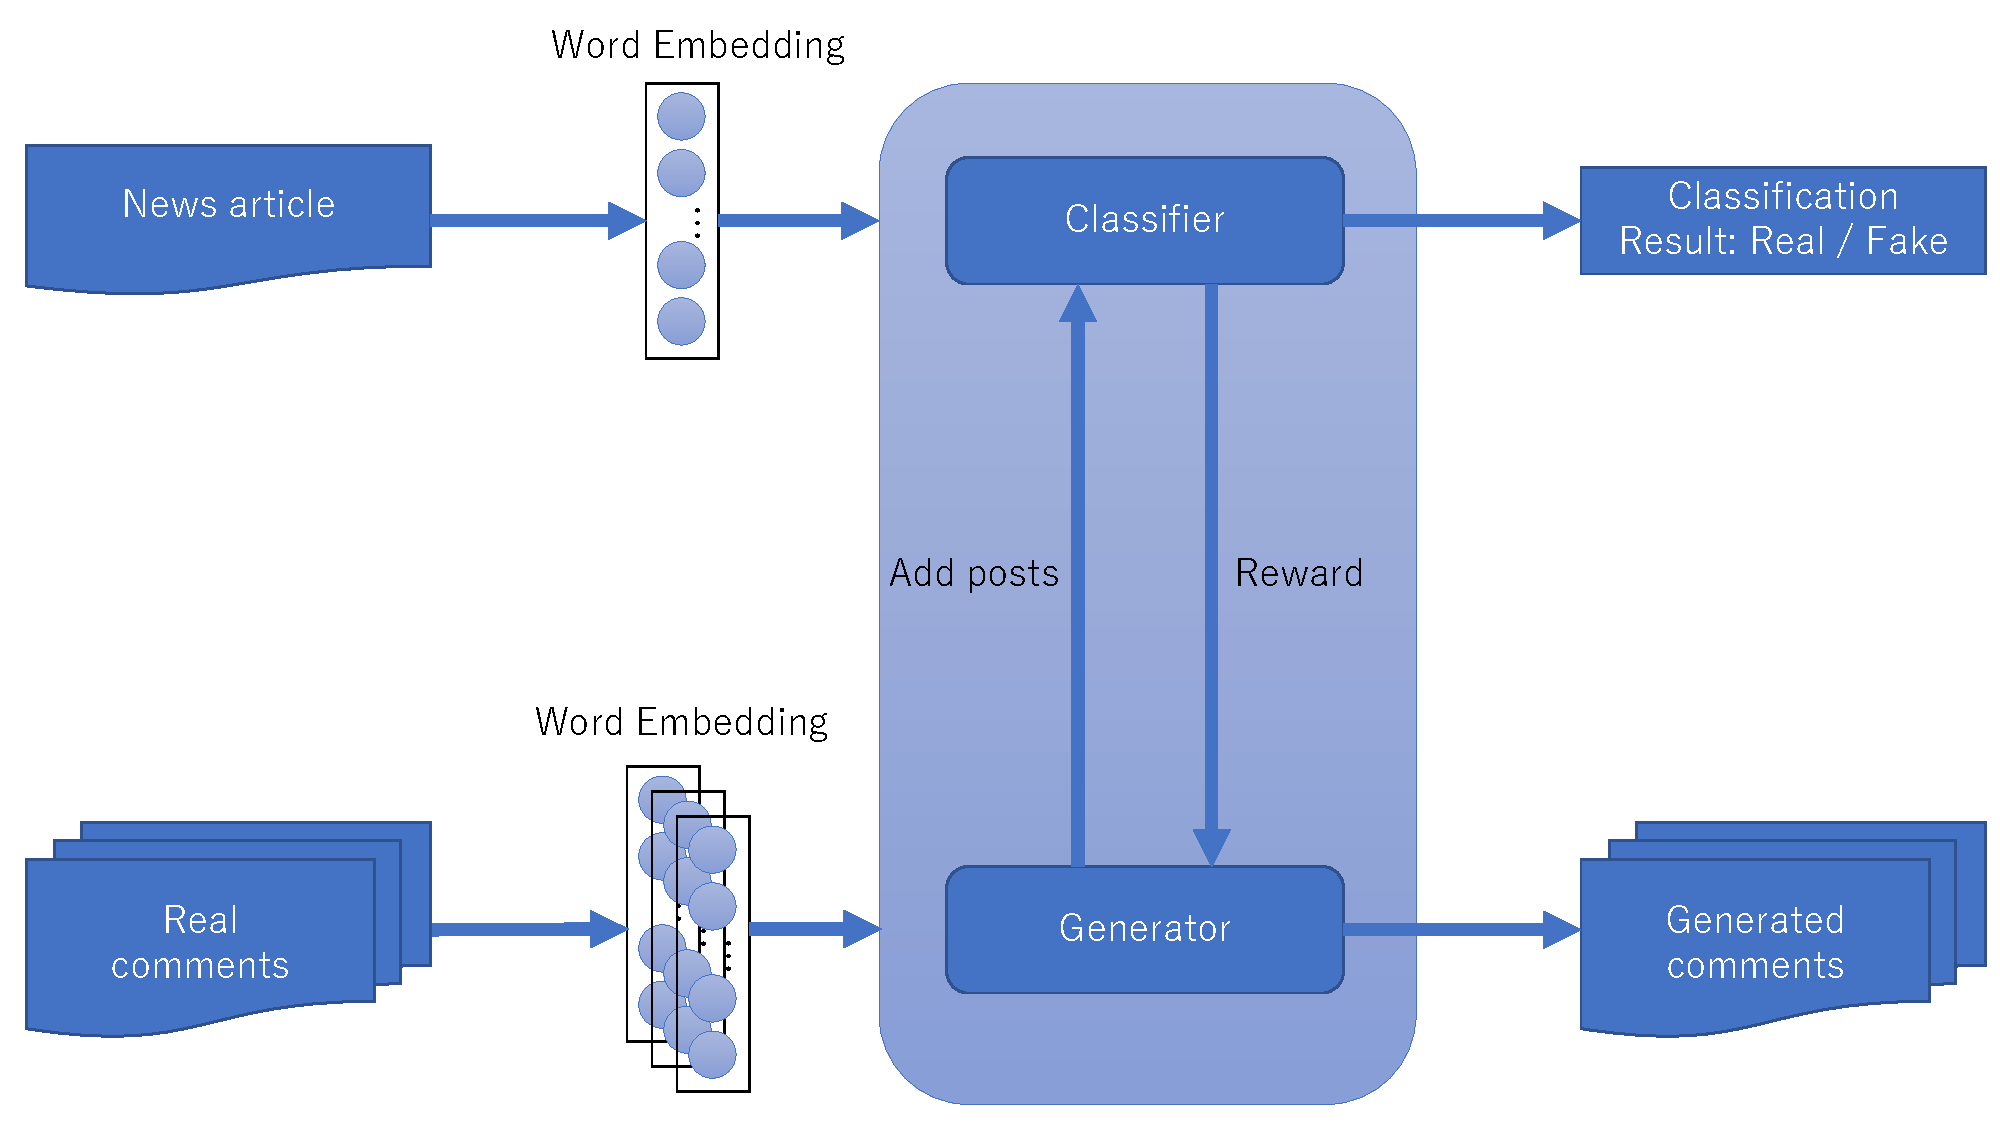
\includegraphics[width=0.85\textwidth]{images/research_proposal_structure.pdf}
    \caption{The structure of our planning proposed model.}
    \label{fig:structure}
\end{figure}

Generator is trained by post feature which is leaked from classifier and
classifier is trained by label of posts(true, fake) and comments(real, generated).
In the test term, classifier only use posts with generated comments in order to
simulate operation on social media.